\documentclass[../main.tex]{subfiles}
\graphicspath{{\subfix{../res/}}}
\begin{document}

Let's begin this implementation by studying our raw dataset (cleaned) and defining the outcomes we want from our system. When these two sections will have been discussed, and choices made, we are going to explore the construct and results from our experimental system.

\subsection{Analysing the raw dataset}
We made a first study of our raw dataset (after some light cleaning of it) to try and understand the data we are working with. First, we wanted to understand the data universe itself. How many entry have we available on our hand. This is the result of this first analysis :
\begin{table}[h]
  \centering
  \begin{tabular}{|c|c|}
    \hline
    Academic Year & Number of Students \\
    \hline
    2018-2019 & 14 \\
    2019-2020 & 13 \\
    2020-2021 & 13 \\
    2021-2022 & 17 \\
    2022-2023 & 32 \\
    \hline
    Total & 90 \\
    \hline
  \end{tabular}
  \caption{Number of Students per Academic Year}
  \label{tab:students_per_year}
\end{table}

Our dataset is small for our need, so we will need to exclude some parts of our conceptual model to test at least our basis hypothesis of being able to cut out dataset into excellence, average and at risk student.
Here is the model we are going to work with for this first implementation, awaiting more data to arrive to test more modules of our system : 

\begin{figure}[H]      
    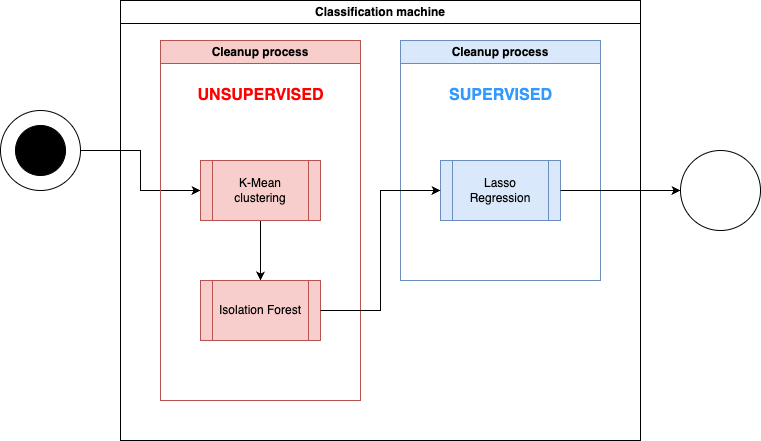
\includegraphics[width=1\linewidth]{res//diagram/simplifiedmdl-Imp_mdl.drawio.png}
    \caption{Simplified algorithmic workflow used in this first implementation.}
    \label{fig:dataworkflow_simp} %lol
\end{figure}

Continuing on our analytical analysis, we wanted to see the average age of our sample using their year of birth available in our dataset. Here is a heatmap of the different academic year and the hotspots by year of birth : 
\begin{figure}[H]      
    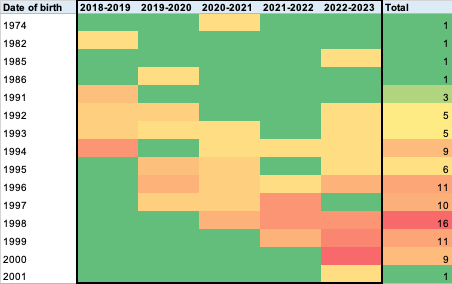
\includegraphics[width=1\linewidth]{res/graph/data_analysis/raw/heatymap_year.png}
    \caption{Heatmap of year of birth by academic year}
    \label{fig:heatmap_dob_acayear}
\end{figure}

As we can see, a strong hotspot is the year 1998 with a frequency of 16 over 90 samples. And, for the academic year 2022/2023, we have another strong hotspot for the year of birth 2000 (with a frequency of 9 over 9 for this year of birth) which indicated all students born in 2000 have registered on the same year (2022/2023).

Another variable we wanted to study is the academic mention obtained by students for each academic year. Thus, giving us a view on which was the best and worst years academically in the dataset.
\begin{figure}[H]      
    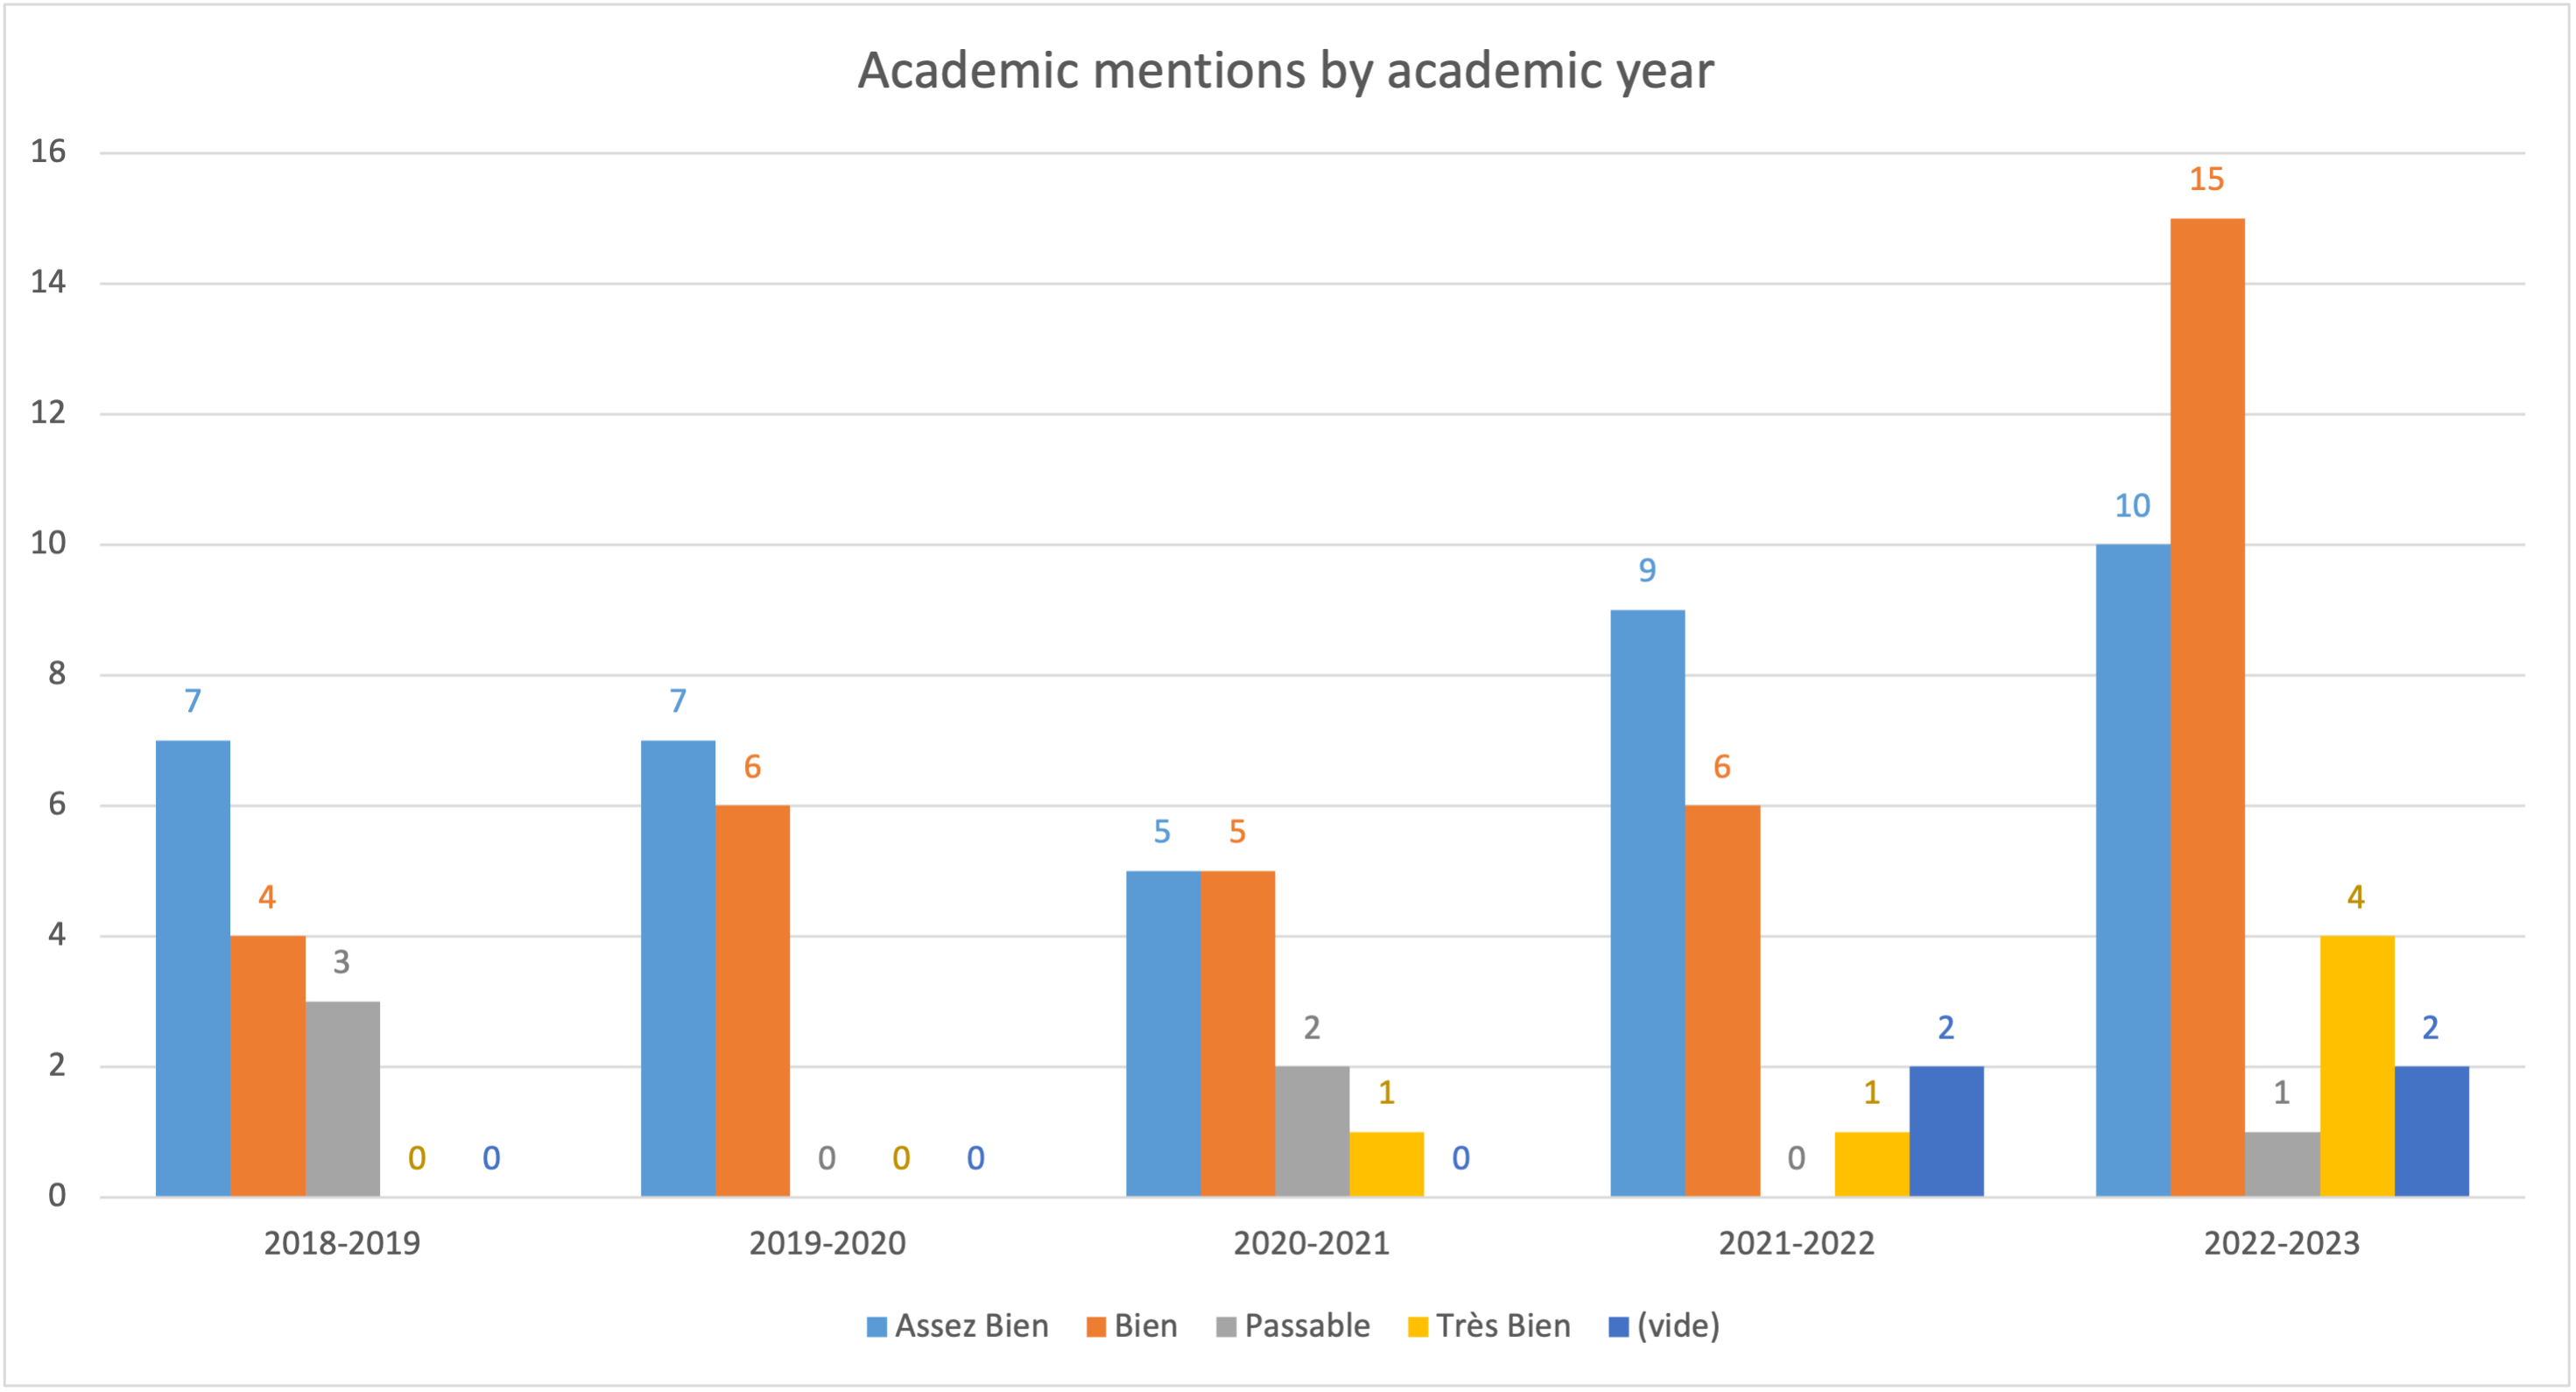
\includegraphics[width=1\linewidth]{res/graph/data_analysis/raw/academicmentions_academic_year.png}
    \caption{Histogram of academic mentions by academic years}
    \label{fig:hist_acament_acayear}
\end{figure}


We can detect one \textit{outlier} for this five available academic years. The year 2022/2023 have been the best year so far with an outstanding 4 \textbf{Très bien} (very good) and 15 \textit{Bien} (good). While the year 2018/2019 lagging behind with 3 students over 14 with a \textit{Passable} mention (only average). However, for both years 2021/2022 and 2022/2023, we have more student with no mention at all.

Finaly, we wanted to see the number of student admitted by year, and do a comparative table of mean of student's final grade for each year. 
\begin{figure}[H]      
    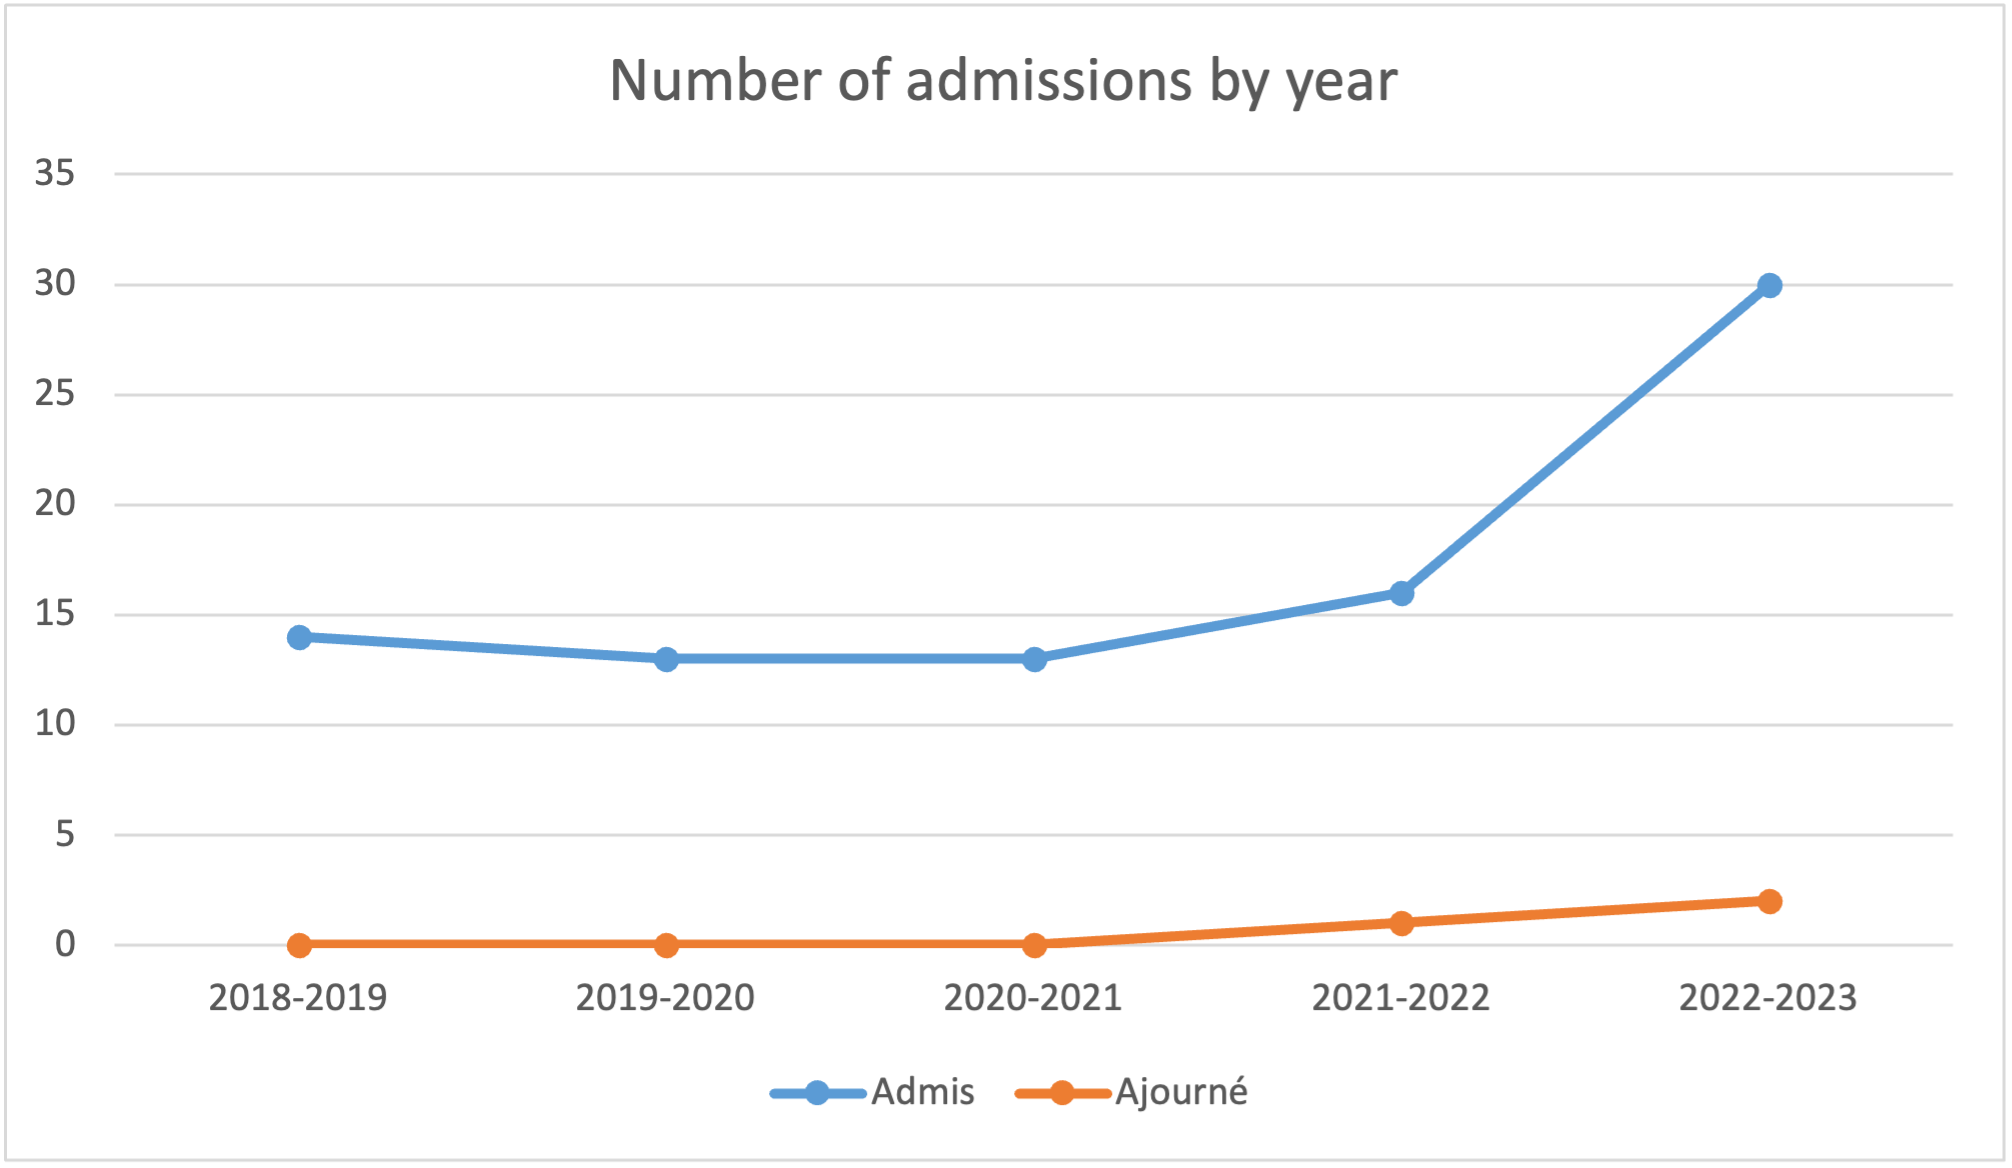
\includegraphics[width=1\linewidth]{res/graph/data_analysis/raw/nbadmissions_year.png}
    \caption{Evolution on the number of admissions by year}
    \label{fig:evol_nb_admis}
\end{figure}
\begin{table}[h]
  \centering
  \begin{tabular}{|c|c|c|c|}
    \hline
    Academic Year & Admited & Adjourned & Total \\
    \hline
    2018-2019 & 12.89 & 0.00 & 12.89 \\
    2019-2020 & 13.82 & 0.00 & 13.82 \\
    2020-2021 & 13.53 & 0.00 & 13.53 \\
    2021-2022 & 13.98 & 11.49 & 13.83 \\
    2022-2023 & 14.41 & 8.67 & 14.05 \\
    \hline
  \end{tabular}
  \caption{Admission Statistics (global grade mean) per Academic Year}
  \label{tab:admission_statistics}
\end{table}

Because our data is not normalized for a \textit{at risk} model, we will only consider predicting the excellence in our dataset with our model.
As we can see, for each year, the global mean is quite similar, orbiting around 13.5/20.

\subsection{Defining the outcomes}

As discussed per our \ref{sec:soa} State of the Art and \ref{sec:analysis} Analysis sections, one hardening point in this kind of study is the definition of success. This broad question needs to be answered before constructing the system as the parameters of it will be influenced by our needed outcomes.
For this first implementation, and according to our available variables and data in our dataset, we will define our success simply based on the final overall grade of the student. Thus, we can define \textbf{our} success as follow :
\begin{quote}
    \textbf{Success :} A student who has follow through the registration correctly, is not dispensed of diploma (forbidden students) and who have an overall grade :
    \begin{equation}
        grade \geq 16
    \end{equation}
\end{quote}

We've chose 16 at the minimum value for success depending on our dataset, which have a maximum of 17 for this variable and to have as much data available to train our system.

\subsection{Building and setting up the system}

From figure \ref{fig:dataworkflow_simp}, we must build a system composed of four different \acrshort{ml} algorithm (\acrfull{knn}, \acrfull{if}, \acrfull{lr}), setted up in order to find definition of success within our dataset. This means creating a profile of excellent student with an average grade of at least 16, not forbidden and with a full registration process completed. 
Then, after training our model, we have to teach him correlations between the profile we have setted-up to train it to find excellency within our registration datasets.




\end{document}